\chapter{Introdução}

%=====================================================

% A introdução geral do documento pode ser apresentada através das seguintes seções: Desafio, Motivação, Proposta, Contribuição e Organização do documento (especificando o que será tratado em cada um dos capítulos). O Capítulo 1 não contém subseções\footnote{Ver o Capítulo \ref{cap-exemplos} para comentários e exemplos de subseções.}.

\section{Contextualização}
Vivemos em um mundo rodeado de tecnologia, onde a cada dia somos surpreendidos com uma coisa totalmente inovadora, disruptiva. Uma era onde a internet foi respons\'avel por atravessar mares, superar dist\^ancias e at\'e mesmo idiomas. Hoje se pode comunicar em tempo real com pessoas que est\~ao em lados completamente oposto ao seu. 

Hoje \'e poss\'ivel que empresas estrangeiras muito distantes fisicamente, como China, India, EUA e etc, forne\c{c}am servi\c{c}os para regi\~oes mais remotas do mundo. Isso inclui servi{c}os de multim\'idia como armazenamento de fotos, de v\'ideos e at\'e conte\'udos de consumo instant\^aneo.

Esse encurtamento de dist\^ancia pode parecer simples, mas vem de um sistema complexo que visa fornecer ao usu\'ario final uma experi\^encia agrad\'avel com conte\'udos entregues de maneira satifat\'oria mas sem, necessariamente, replic\'a-lo por todo o globo. O que nos leva a dizer que uma CDN (\textit{Content Delivery Network}) \'e uma rede de distribui\c{c}\~ao de conte\'udo que tem como objetivo fornecer ao usu\'ario de aplica\c{c}\~oes globais uma experi\^encia satisfat\'oria na utiliza\c{c}\~ao de servi\c{c}os, principalmente sob demanda. Podemos ver alguns desses servi\c{c}os na figura \ref{figura:contextualizacao}.
\begin{figure}[H]
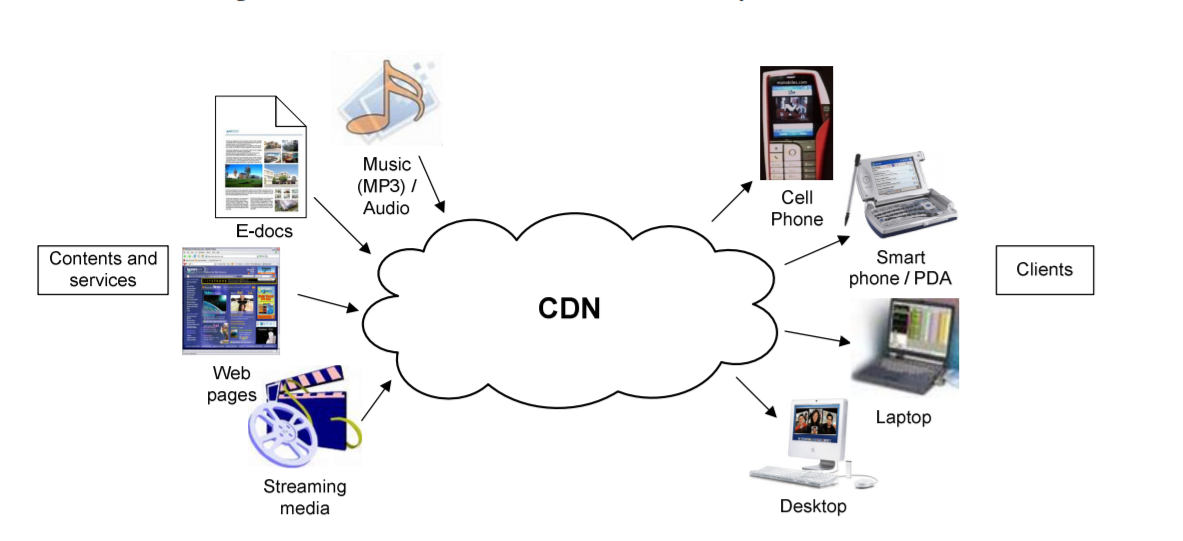
\includegraphics[height=7cm]{Figuras/contextualizacao.png}
\caption{Fornecedores x Consumidores} 
\label{figura:contextualizacao} 
\end{figure}
H\'a v\'arios servi\c{c}os que se utiliza no dia a dia onde essa no\c{c}\~ao de CDN \'e completamente abstrata ao usu\'ario final, como servi\c{c}os de Video-On-Demand de empresas de TV, spotify, Amazon Prime Video e at\'e Netflix, como \'e mostrado no artigo do \cite{adhikari2012unreeling}.

Existem hoje diversas empresas que fornecem esse servi\c{c}o ao redor do globo. Como Akamai, Limelight, Level 3 entre outras. Dessas redes a mais conhecida \'e a Akamai, que foi criada dentro do MIT (\textit{Massachusetts Institute of Technology}), e tem como clientes empresas como Adobe, \emph{Airbnb}, \emph{American Idol}, \emph{Audi} e muitas outras. Essas tr\^es redes s\~ao hoje as principais fornecedoras de servi\c{c}o de CDN. Cada uma com uma caracter\'istica e voltada para um p\'ublico.
\section{Problema}

Falar da questão de segurança e dificuldade de se garantir a segurança de um conteúdo que é distribuído em multiplas máquinas.
\section{Objetivos}

Resumidamente: Aprensentar uma solução que permite cifrar um conteúdo com a chave privada do fornecedor de conteúdo de forma que possa ser decifrado por qualquer usuário que tenha autorização.
\section{Estrutura do Documento}

Apresentar a estrutura do documento - Fazer por ultimo.
%=====================================================
